\begin{abstract}
	The performance characteristics of a software system depends to a significant extent on its configuration and workload. State-of-the-art performance modeling approaches either address configuration-dependent or workload-dependent performance behavior.  The interaction of both factors and how they influence performance have not been systematically studied so far. Understanding to what extent configuration and workload---individually and combined---cause a software system’s performance to vary is key to understand whether performance models are generalizable, across different configurations and workloads. Assessing the impact and driving factors of such input sensitivity is key to develop strategies that obtain representative performance prediction models.
	
	To shed light on this issue, we have conducted a \emph{systematic} empirical study, analyzing a multitude of configurations and workloads across ten software systems. We have obtained a substantial number of black-box performance measurements and enriched them with coverage data to assess whether and how configuration choices and workloads interact and shape software performance. 
	We find that code coverage (i.e., \textit{what} code is executed) and code utilization (i.e., \textit{how} covered code is executed) are driving factors for workload-specific performance differences. Beyond code coverage testing, our findings motivate the use of dynamic code analyses to identify whether and in which way configuration options are sensitive to varying the workloads.
\end{abstract}

\section{Introduction}

%\paragraph*{\color{purple}Context}
Most modern software systems can be customized via configuration options to meet user demands. Configuration options can enable desired functionality or tweak non-functional aspects of a software system, such as improving performance or energy consumption. The relationship of configuration choices and their influence on performance has been extensively studied in the literature~~\cite{dorn2020,siegmundPerformanceinfluenceModelsHighly2015,haDeepPerf2019,perfAL,guoVariabilityawarePerformancePrediction2013,sarkarCostEfficientSamplingPerformance,guo_2018_data,fourier_learning_2015,perLasso}. The backbone of performance estimation are prediction models that map a given configuration to the estimated performance value. Learning performance models relies on a training set of configuration-specific performance measurements. In state-of-the-art approaches observations usually employ only a single workload which aims at emulating a specific real-world application scenario.

The choice of the workload (i.e., the input fed to the software system) is known to influence the performance of configurable software systems in different ways as has been shown for the domains of SAT solvers~\cite{falkner_sat_solvers_2015,satzilla_2008}, compilation~\cite{ding_compilation_2015,plotnikov_compilation_2013}, video transcoding~\cite{maxiaguine_workload_2004,alves_sampling_2020}, data compression~\cite{khavari_compression_2019}, and code verification~\cite{koc_satune_2021}. Besides apparent interactions, such as performance scaling with the size of a workload, qualitative aspects can result in more complex and non-trivial performance interactions. For instance, \citeauthor{alves_sampling_2020} have shown that the video transcoder \textsf{x264} exhibits different performance distributions depending on the video source file~\cite{alves_sampling_2020}, and \citeauthor{liao_2020_using_emse} have confirmed this for stream processing applications~\cite{liao_2020_using_emse}. As varying the workload adds another layer of complexity to modeling performance, we cannot guarantee that performance models trained with a single workload \textit{generalize} to arbitrary workloads and make meaningful estimations. 

%\paragraph*{\color{purple}Motivation}
To address this limitation, two different directions have been pursued in the literature. First, performance models trained using a specific workload can be adapted to another specific workload~\cite{jamishidi_transfer_2017,jamshidi_learning_2018,jamshidi_transfer_gp_2017}. Second,  one can specify workload characteristics as further independent variables when modeling configuration-dependent performance~\cite{koc_satune_2021}.
The first strategy direction relies on transfer learning techniques, where, given an existing performance model, in a separate step only the differences to a new environment are learned. Such a transfer function encodes which configuration options’ influence on performance is sensitive to workload variation. While transfer learning is an effective strategy that is not limited to varying workloads~\cite{jamshidi_learning_2018}, but can also be applied to different versions~\cite{jamishidi_transfer_2017,jamshidi_transfer_gp_2017,martin_transfer_2021}, or hardware setups~\cite{ding_bayesian_2020}, its main limitation is that the transfer function is specific to the differences between two environments.

In contrast to transfer learning, a more generalist approach is to consider the input fed to a software system as a further dimension for modeling performance. Here, a workload can be characterized by properties that---individually or in conjunction with software configuration options---influence performance. For such a strategy to work, one requires knowledge of the characteristics of a workload that influence performance. This strategy has been effectively tested for a  variety of application-domains, such as program verification~\cite{koc_satune_2021}. However, the added complexity comes at significant cost. 
Not only does this require substantially more measurements, we often lack knowledge of which performance-relevant characteristics best describe workloads.
 
%\paragraph*{\color{purple}Problem}
The existing body of research reflects the prevalence and importance of the workload influence on software systems~\cite{khavari_compression_2019,maxiaguine_workload_2004,plotnikov_compilation_2013,ding_compilation_2015,falkner_sat_solvers_2015,satzilla_2008,alves_sampling_2020}. All these works are aware of the workload dimension as a factor of performance variation, yet little is known about the quality and driving factors of the \emph{interplay} between configuration options and workloads. Our understanding of this cross-factor relationship lacks knowledge of the following aspects:

\begin{compactitem}
	\item How different is configuration-specific performance across different workloads? 
	\item How many configuration options are responsible for differences in workload-specific performance behavior?
	\item What are the driving factors of the interplay between configuration options and workloads with regard to performance? 
\end{compactitem}

To answer these questions, we have conducted a systematic empirical study that sheds light on whether and how configuration options and workload choices interact with regard to performance. 
Specifically, we analyze 29\,347 configurations and 55 workloads across six configurable software systems to obtain a broad picture of the interaction of configuration and workload when learning performance models and estimating a configuration's performance (i.e., response time). Aside from studying the sole effects of workload variation on performance behavior, we explore possible driving factors. To this end, we enrich performance observations with corresponding statement coverage data to understand workload variation at finer granularity.

Our findings show that varying the workload can influence con\-fi\-gu\-ra\-tion-de\-pen\-dent software performance in different ways, including non-linear and non-monotonous effects. Our findings suggest that (a) coverage of code  specific to configuration options as well as (b) how such code is utilized are driving factors of input sensitivity. A key insight is that, to maintain and improve performance model representativeness, an additional notion of input sensitivity has to be considered. We argue that the use of code analysis techniques to address input sensitivity when varying the workload and maintain and improve the representativeness of a performance-prediction model.

To summarize, we make the following contributions: 

\begin{compactitem}
	\item An empirical study of 29\,347 configurations and 55 workloads across six configurable software systems on whether interactions of workloads with configuration options affect performance and what factors can drive such interactions;
	
	\item A detailed analysis that illustrates that variation in code coverage and code utilization due to varying workloads can affect the influence of configuration options on software performance; 
	
	\item A companion Web site\footnote{\url{https://github.com/fse-submission-2022/workload-performance/}} with supplementary material including performance and coverage measurements, experiment workloads and configurations, and an interactive dashboard\footnote{\url{https://workload-performance.herokuapp.com/}} for additional visualizations left out due to space limitations.
\end{compactitem}




\section{Background and Problem Statement}
\subsection{Performance Prediction Models}~\label{sec:perfmodels}
Configurable software systems are an umbrella term for any kind of software system that exhibits configuration options to customize functionality. While the primary purpose of configuration options is to select and tune functionality, each configuration choice may also have implications on non-functional properties---be it intentional or unintentional. 
%There are different approaches to capture the relationship between configuration options and performance indicators, most basically either \emph{analytical} or \emph{empirical} in nature. All share the objective to 
All performance prediction models approximate non-functional properties, such as execution time or memory usage, as a function of software configurations $c \in C$, formally $\Pi: C \rightarrow \mathbb{R}$. 

%Analytic models incorporate existing knowledge about the operations of a software system, comparable to estimating an algorithm’s complexity~\cite{analytic_model_2000,analytic_model_2011}. Here, one deliberately includes or excludes configuration options as predictors and selects a model structure following the current understanding of the software system. While it avoids ambiguity in terms of feature selection and explainability, analytic approaches do not guarantee to cover unanticipated idiosyncrasies or interactions between configuration options.

Such models do not rely on an understanding of the internals of a configurable software system, but are learned from a training set of configuration-specific performance observations. In this vein, finding configurations with optimal performance~\cite{nairUsingBadLearners2017,nairFlash18,ohFindingNearoptimalConfigurations2017} and estimating the performance for arbitrary configurations of the configuration space is an established line of research~\cite{siegmundPerformanceinfluenceModelsHighly2015,haDeepPerf2019,perfAL,guoVariabilityawarePerformancePrediction2013,sarkarCostEfficientSamplingPerformance,guo_2018_data,fourier_learning_2015,perLasso}.
Over the past years, several different machine-learning techniques, including probabilistic programming~\cite{dorn2020}, multiple linear regression~\cite{siegmundPerformanceinfluenceModelsHighly2015}, classification and regression trees~\cite{guoVariabilityawarePerformancePrediction2013,sarkarCostEfficientSamplingPerformance,guo_2018_data}, Fourier learning~\cite{fourier_learning_2015,perLasso}, and deep neural networks~\cite{haDeepPerf2019,perfAL} have shown effective to learn configuration-dependent software performance.
The set of configurations for training can be sampled from the configuration space using a variety of different sampling techniques~\cite{kaltenecker_interplay_2020}. All sampling strategies aim at yielding a representative sample, either by covering the main effects of configuration options and interactions among them~\cite{siegmundPredictingPerformanceAutomated2012}, or sampling uniformly from the configuration space~\cite{ohFindingNearoptimalConfigurations2017,kaltenecker_distance-based_2019}.
Most approaches share the perspective of treating a configurable software system as a black-box model at application-level granularity. Recent work has incorporated feature location techniques to guide sampling effort towards relevant configuration options~\cite{velez_2020_configcrusher_jase,velez_comprex_2021} or model non-functional properties at finer granularity~\cite{weber_white_2021,han_confprof_2021}.

{\color{black}
\subsection{Varying Workloads}\label{sec:varying_workloads}
%\subsubsection{Whats is a workload?}
When assessing the performance of a software system, we ask how well a certain \textit{operation} is executed, or, phrased differently, how well an \textit{input fed to the software system} is processed. Such inputs, commonly called workloads, are essential to assessing performance, even detached from the specific context of configurable software systems. By nature, the workload of a software system is application-specific, such as a series of queries and transactions fed to a database system, a set of raw image files for video encoding, or an arbitrary file for data compression etc. Workloads can often be distinguished by characteristics (dimensions) they exhibit, such as their file size in general, or, the  type of data to be compressed (text, binary data) for instance.

%\subsubsection{Workload Characterization}\label{sec:workload-characterization}
A useful workload for assessing performance or benchmarking should, in practice, closely represent the real-world scenario that the system under test is deployed in. To achieve this, a well-defined and widely employed technique in performance engineering is workload characterization~\cite{ceesay2020,papadopoulos2021}. To select a representative workload, it is imperative to explore workload characteristics and validate a workload with real-world observations. This can be achieved by constructing workloads, among others, from usage patterns~\cite{calzarossa2016}, or by increasing the workload coverage by using a mix of different workloads rather than a single one~\cite{jiang2015survey}.

While workload characterization and benchmark construction is domain-specific, there are numerous examples of this task being driven by community efforts instead of individuals. For instance, the non-profit organizations Standard Performance Evaluation Corporation (SPEC) and Transaction Processing Performance Council (TPC) provide large bodies of benchmarks for data-centric applications or across different domains, respectively.

\subsection{Representative Estimations?}\label{sec:generalizability}
While the notion of representative workloads is ubiquitous in an industry setting, we face a different situation in research on empirical performance models (cf. Section~\ref{sec:perfmodels}): Most approaches provide accurate performance estimations, yet are based on observations gained by varying configurations while keeping the workload the same. The choice of workloads is an "orthogonal" problem~\cite{han_confprof_2021} and can limit the model's generalizability to different workloads, especially if the training workload poorly represents real-world scenarios. While the configuration-specific behavior might be congruent across different workloads (i.e, a configuration scoring comparably for different workloads), we cannot rely on such assumptions in practice, where different workloads can indeed result in entirely different configuration-specific performance behavior.

\begin{figure}
	\centering\footnotesize
	\begin{tabular}{r|rrr|rr}
		\toprule
		id & $c_1$ & $c_2$ &  $c_3$ & $\Pi_{w_1}(c)$ & $\Pi_{w_2}(c)$\\
		\midrule
		1  & \cellcolor{black!15}1 & \cellcolor{black!4}0 & \cellcolor{black!4}0 & \cellcolor{green!10}4 seconds & 22 seconds \\
		2  & \cellcolor{black!4}0 & \cellcolor{black!15}1 & \cellcolor{black!4}0 & 6 seconds & \cellcolor{green!10}14 seconds \\
		3  & \cellcolor{black!4}0 & \cellcolor{black!4}0 & \cellcolor{black!15}1 & 9 seconds & 35 seconds \\
		\bottomrule
	\end{tabular}
	
	$$ \Pi_{w_1}(c) ~=~ c_1 \times 3 ~+~ c_2 \times 5 ~+~ c_3 ~\times 8 ~+~ 1$$
	$$ \Pi_{w_2}(c) ~=~ c_1 \times 21 ~+~ c_2 \times 13 ~+~ c_3 \times 34 ~+~ 1$$
	\caption{Input sensitivity in the case for a software system with three configuration options $C = (o_1, o_2, o_3)$.}
	\label{fig:sensitivity_example}
\end{figure}


{\color{blue!80!black} Consider the illustratory example from Figure~\ref{fig:sensitivity_example}. Here, we measure performance under three different configurations and two different inputs $w_1$ and $w_2$. Apparently, the software system takes longer for $w_2$, regardless of the configuration. This could, for instance, be attributed to $w_2$ being more complex and performance scaling proportionally. However, if we ask which option is fastest in general there is no concrete answer since configuration 1 prevails for $w_1$ and configuration 2 for $w_2$. If we look at the corresponding performance prediction models below, we learn that the influence of $o_1$ is smaller than for $o_2$ in $\Pi_{w_1}$ and vice versa in $\Pi_{w_2}$. Thus, there must be some hidden feature or variable, the "difference" between $w_1$ and $w_2$ that accounts for this performance variation beyond configuration options.
}
%{\todo{kürzen, Beispiel für performance model hier bringen}\color{red}Revisiting an observation by Pereira\,et al.~\cite{alves_sampling_2020}, the following example illustrates that even seemingly small differences in the composition of a workload can induce performance behavior that is hard to anticipate: We tested the performance (throughput: transactions per second) of a number of configurations for the database system \htwo across two different workloads. Both workloads are instances of the database benchmark \textsf{TPC-C}, consisting of a fixed-ratio mix of transactions (inserts, updates, selects) for a specific database schema. The only difference was varying the scale factor, which controls for the number of warehouses modeled in the schema. The resulting performance distributions are given in Figure~\ref{fig:h2_intro}.

%While one might first expect that a more complex workload results in lower throughput, this is indeed the case, but does not hold for all configurations. The median throughput decreases for the larger number of warehouses, yet the shape and spread of the distribution are entirely different. Most notably, the maximum throughput for the greater scale factor is higher than for the smaller scale factor, indicating that some configurations indeed do not follow the general trend. This illustrates that the effect of varying the workload for some configurations cannot be captured by a linear transformation (constant shift or scaling).}


Some aspects of this \emph{input sensitivity} have been observed and documented before in the literature~\cite{liao_2020_using_emse,alves_sampling_2020,jamishidi_transfer_2017} and raise questions, such as: \textit{Which options are input sensitive? What are the driving factors for input sensitivity? Can we estimate which options are input-sensitive?} We set out to answer these questions in this paper.
	
\subsection{Workloads and Performance Prediction} ~\label{sec:strategies}
To some aspects of the said questions, different approaches have been proposed to tackle the problem of input sensitivity.

\paragraph{Workload-aware Performance Modeling}\label{sec:workload-aware}
Extending on workload characterization (cf.~Section~\ref{sec:varying_workloads}), a strategy that embraces workload diversity is to incorporate workload characteristics into the problem space of a performance prediction model. Here, performance is modeled as a function of both the configuration options exhibited by the software system as well as the workload characteristics, formally $\Pi: C \times W \rightarrow \mathbb{R}$.
The combined problem space enables learning performance models that generalize to workloads that exhibit characteristics denoted by $W$ since we can screen for performance-relevant combinations of options and workload characteristics. Although this strategy is highly application-specific, it has been successfully applied to different domains, such as program verification~\cite{koc_satune_2021}. However, its main disadvantages are twofold: The combined problem space (configuration and workload dimension) requires substantially more observations to screen for identifying performance-relevant options, characteristics, and combinations thereof. In addition, previous work  found that  only few configuration options are input sensitive~\cite{jamishidi_transfer_2017} when varying the workload. That is, the problem of identifying meaningful, but sparse predictors is exacerbated since one must not only identify performance-relevant configuration options, but also input-sensitive ones.

\paragraph{Transfer Learning for Performance Models}\label{sec:transfer}
Another strategy that builds on the fact that, across different workloads, only few configuration options are in fact input sensitive~\cite{jamishidi_transfer_2017}. Here one first trains a model on a standard workload and, subsequently, adapts it to different workloads. Contrary to a generalizable workload-aware model, transfer learning strategies focus on approximating a transfer function that, without characterizing the workload, encodes the information of which configuration options are sensitive to differences between a source and target pair of workloads. Training a workload-specific model and adapting it on occasion provides an effective means to reuse performance models, which is not limited to workloads~\cite{jamshidi_learning_2018}, but has successfully been applied to different hardware setups~\cite{ding_bayesian_2020,valov_transferring_performance_2017} and across versions~\cite{martin_transfer_2021}. The main shortcoming of transfer learning approaches is that they do not generalize to arbitrary workloads, since a transfer function is tailored to a specific target workload. Here, one trades off generalizability and measurement cost as learning a transfer function requires substantially fewer training samples.

While both directions are effective means to handle input sensitivity, to the best of our knowledge, there is no \textit{systematic} assessment of the factors that drive the interaction between configuration options and workloads with regard to performance. Understanding scenarios that are associated with or even cause incongruent performance influences across workloads can help practitioners to employ established analysis techniques more effectively and can motivate researchers to devise analysis techniques dedicated to such scenarios.
}
\section{Study Design}~\label{sec:study}
In what follows, we describe the general experiment setup and study design as well as research questions. We make all performance measurement data, configurations, workloads, and learned performance models available on the paper's companion Web site.
\subsection{Research Questions}
Our first two research questions shed light on the input sensitivity of the performance behavior of the studied software systems. We first take a look at systems as a whole~(\RQref{1}) with regard to a large set of configurations and, subsequently, consider individual configuration options~(\RQref{2}). Extending on the results of \RQref{2}, we explore possible driving factors and indicators for workload-specific performance variation~(\RQref{3}).

\subsubsection{Performance Variation Across Workloads}
Performance variation can arise from differences in the workload~\cite{benchmarking_book}. In a practical setting, the question arises whether, and if so, to what extent an existing workload-specific performance model is representative of the performance behavior of other workloads. 
That is, can a model estimating performance of different configurations be reused for the same software system but run with a different workload? Depending on the degree of similarity of the performance behavior across workloads, we obtain a clearer picture of the prevalence of input sensitivity and to what extent the strategies outlined in  Section~\ref{sec:strategies} might be applicable.
To this end, we formulate the following research question: 

\RQ{1}{To what extent does \textit{performance behavior} vary across workloads?}
\subsubsection{Option Influence Across Workloads}
At large, performance behavior is the resulting effect arising from multiple configuration options’ and combinations’ respective influences. To understand which configuration options are driving performance variation, in general, and which are input sensitive, in particular, we formulate the following research question:

\RQ{2}{To what extent do \textit{influences of individual configuration options} depend on the workload?}
\subsubsection{Causes of Input Sensitivity}
The first two research questions describe the performance behavior of our subject systems: Based on the results of related work, we expect configuration options to be, at least, to some extent input sensitive. To contextualize our findings, we switch our perspective to the code level. The goal is to understand the relationship between input sensitivity (i.e., variation in the performance influence of configuration options) and the execution of the subject system under varying workloads. We hypothesize that executions under different workloads also exhibit variation with respect to what code sections are executed and how this code is used. Using code coverage analysis---an easy to understand and widely employed technique---we are interested in how far one could infer or explain performance influence variation just based on code. 

\RQ{3}{Does the variation in configuration options' performance influence across workloads correlate with differences in the respective execution footprint?}
\subsection{Experiment Setup}\label{sec:setup}
\subsubsection{Subject System Selection}
We selected ten configurable software systems for our study. To ensure that our findings are not specific to one domain or ecosystem, the selection comprises an equal mix of Java and C/C++ systems from different application domains (cf. Table~\ref{tab:subject_systems}). We include systems studied in previous and related work~\cite{velez_2020_configcrusher_jase,weber_white_2021,alves_sampling_2020} and incorporate further ones with comparable size and configuration complexity. All systems operate by processing a domain-specific input fed to them (henceforth called \textit{workload}). This study treats execution time as the key performance indicator with the exception of \htwo, where we report throughput.

\begin{table}
	\footnotesize
	\centering
	\caption{Subject System Characteristics}
	\begin{tabularx}{\linewidth}{lllrrrr}
		\toprule
		\textbf{Software System} &  \textbf{Application Type} & \textbf{Revision} & \textbf{ \#\,O} & \textbf{\#\,C} & \textbf{\#\,W}  \\
		\midrule
		\jumper & Audio encoder & 1.0.4 & 19 & 4\,196 & 6   \\
		
		\kanzi & File compressor & 1.9 & 24 & 4\,112 & 9 \\
			
		\dconvert & Image scaling & 1.0.0-alpha7 & 17 & 6\,764 & 12  \\
				
		\htwo & Embedded database & 1.4.200 & 16 & 1\,954  & 8  \\
		
		\batik & SVG rasterizer & 1.14 & 10 & 1\,919 &  11  \\
		
		\jadx & Java decompiler & 1.2.0 & 18 & 10\,502 & 9  \\
\bottomrule

\end{tabularx}\\
{\vspace{1mm}\textit{Abbreviations: \#\,O: No. of options, \#\,C: No. of configurations, \#\,W: No of. workloads}}

	\label{tab:subject_systems}
\end{table}

\subsubsection{Workload Selection}
This study relies on a selection of workloads for each domain or software system. Ideally, each set of workloads is diverse enough to be representative of most possible use cases. We selected the workload sets in this spirit, but cannot always guarantee a measurable degree of diversity and representativeness. This is due to the opacity of workloads: Beyond educated guesses, prior to conducting measurements, it is not possible to state which workload characteristics (size, scale, file type etc.) are performance-relevant. We discuss this aspect in the threats to validity. Below we outline the ten case studies along with the workloads tested. 
%All workloads and resources are made available on the paper’s companion Web site.


For the \textit{audio encoder} \jumper, the measured task was to encode raw WAVE audio signals to MP3 (\jumper). We selected a number of different audio files from the Wikimedia Commons collection\footnote{\url{Link to wikimedia}} and aimed at varying the file size/signal length, sampling rate, and number of channels. Both applications share all workloads.

For the \textit{video encoder} \xzwo, the measured task was to encode raw video frames (y4m format). We selected a number of files from the “derf collection”\footnote{\url{https://media.xiph.org/video/derf/}}, a set of test media for a variety of use cases. The frame files vary in resolution (low/SD up to 4K) and file size. For files with 4K resolution, we limited our measurements to encoding a subset of consecutive frames.

For the \textit{file compression} tools \kanzi, \xz, and \lrzip, we used a variety of community compression benchmarks that represent different goals, including mixes of files of different types (text, binary, structured data etc.) or single-type files. We augmented this set of workloads with custom data, such as the Hubble Deepfield image and a binary of the Linux kernel. Beyond this set of workloads, for \xz and \lrzip we added different parameterizations of the UIQ2 benchmark\footnote{\url{link zu uiq2 benchmark}} to study the effect of varying file size. 

For the \textit{SMT solver} \zdrei, the measured task was to decide the satisfiability (find a solution or counter example) of a range of logical problems expressed in the SMT2 format. We selected the six longest-running problem instances from z3’s performance test suite and augmented it with additional instances from the SMT2-Lib repository\footnote{\url{Link to SMT2-Lib}} to cover different types of logic and increase diversity.

For the \textit{SVG rasterizer} \batik, the measured task was to transform a SVG vector graphic into a bitmap. We selected a number of resources from the Wikimedia Commons collection, primarily varying the file size.

For the embedded \textit{database} \htwo, we used a selection of four benchmarks (SmallBank, TPC-H, YCSB, Voter) from \textsc{OLTPBench}~\cite{difallah_oltp_2013}, a load generator for databases that allows for using a variety of performance testing benchmarks. For each benchmark, we varied the scale factor, which controls the complexity (number of entities modeled) in each scenario.

For the \textit{Java decompiler} \jadx, the measured task was to decompile a number of Android applications in DEX byte code. We selected a number of APK packages from APKMirror\footnote{\url{https://apkmirror.com/}} from different domains (social media, games, utility etc.) and of varying size.

For the \textit{image scaler} \dconvert, the measured task was to transform resources (image files, Photoshop sketches) at different scales (useful for Android development). We selected files that reflect \dconvert's documented input formats (JPEG, PNG, PSD, and SVG) and vary in file size.


\subsubsection{Configuration Sampling}\label{sec:sampling}
For each subject system, we sampled a set of configurations. As exhaustive coverage of the configuration space is infeasible due to combinatorial explosion~\cite{henardCombining2015}, for binary configuration options, we combine several coverage-based sampling strategies and uniform random sampling into an \emph{ensemble} approach: 
We employ option-wise and negative option-wise sampling~\cite{siegmundPerformanceinfluenceModelsHighly2015}, where each option is enabled once (i.e., in, at least, one configuration), or all except one, respectively. In addition, we use pairwise sampling, where two-way combinations of configuration options are systematically selected. Interactions of higher degree could be found accordingly, however, it is computationally prohibitively expensive~\cite{henardCombining2015}. 
Last, we augment our sample set with a random sample that is, at least, the size of the coverage-based sample. To achieve a nearly uniform random sample, we used \emph{distance-based sampling}~\cite{kaltenecker_distance-based_2019}. If a software system exhibited numeric configuration options, we varied them across, at least, two levels to account for their effect. %All variability models and sample sets can be found on the companion Web site.


\subsubsection{Coverage Profiling}\label{sec:profiling}
To assess what lines of code are executed for each combination of workload and software configuration, we used two separate approaches for Java and C/C++. For Java, we used the on-the-fly profiler \textsc{Jacoco}\footnote{\url{https://www.jacoco.org/jacoco/trunk/doc/}} that intercepts byte code running on the JVM at run-time. For C/C++, we added instrumentation code to the software systems using \textsc{Clang/LLVM}\footnote{\url{link to LLVM}} to collect coverage information. We split the performance measurement and coverage analysis runs to  avoid distortion from the profiling overhead.

	
\subsubsection{Measurement Setup}\label{sec:measurement_setup}
All experiments were conducted on three different compute clusters), where all machines within a compute cluster had the identical hardware setup: Cluster \textsf{A} with an Intel Xeon E5-2630v4 CPU (2.2\,GHz) and 256\,GB of RAM, cluster \textsf{B}  with an Intel Core i7-8559U CPU (2.7\,GHz) and 32\,GB of RAM, and cluster \textsf{C} with an Intel Core i5-8259U (2.3\,GHz) and 32\,GB of RAM. All clusters ran a headless Debian 10 installation (kernel 4.19.0-17 for cluster \textsf{A} and 4.19.0-14 for clusters \textsf{B} and \textsf{C}). To minimize measurement noise, we used a controlled environment, where no additional user processes were running in the background, and no other than necessary packages were installed. 

We ran each subject system \textit{exclusively} on a single cluster: \htwo on cluster \textsf{A}; \dconvert, \batik and \jadx on cluster \textsf{B}; the remaining systems on cluster \textsf{C}.

For all data points, we report the median across five repetitions (except for \htwo), which has shown to be a good trade-off between variance and measurement effort. For \htwo, we omitted the repetitions as, in a pre-study, running on the identical cluster setup, we found that across all benchmarks the coefficient of variation of the throughput was consistently below 5\,\%.



\section{Study Results}~\label{sec:results}
\subsection{Comparing Performance Distributions ($RQ_1$)}\label{sec:rq1}
\subsubsection{Operationalization}
We answer \RQref{1} by pairwisely comparing the performance distributions from different workloads (cf. the comparison in Figure~\ref{fig:h2_intro}) and by determining whether any two distributions are similar or, if not, can be transformed into each other: For the former case, we tested all combinbations of workload-specific performance observations with the Wilcoxon signed-rank test\footnote{We use non-parametric methods since performance-distributions are often long-tailed and multi-modal~\cite{curtsinger_stabilizer_2013,maricq2018taming} and, thus, fail to meet requirements for parametric methods.}~\cite{lovric_international_2010}. For all combinations, we rejected the null hypothesis $H_0$ at $\alpha=0.95$. To account for overpowering due to high and different sample sizes (cf. Table~\ref{tab:subject_systems}), we further checked effect sizes to weed out negligible effects. Following the interpretation guidelines from Romano et al.~\cite{romano2006exploring}, for no combination, Cliff's~$\delta$~\cite{Cliff1993DominanceSO} exceeded a threshold effect size of $\vert\delta > 0.147\vert$.
For the latter case, we are specifically interested in what \textit{type} of transformation is necessary as this determines \textit{how} complex a workload interacts with configuration options. Specifically, we categorize each pair of workloads with respect to the following aspects: 

\begin{compactenum}

	\item \textit{Linear Correlation}: To test whether both performance distributions are shifted by a constant value or scaled by a constant factor, we compute for each pair of distributions Pearson's correlation coefficient $r$. To discard the sign of relationship, we use the absolute value and a threshold of $\vert r\vert >0.6$ to indicate a linear relationship.
	
	\item \textit{Monotone Correlation}: Finally, we test whether there exists a monotonous relationship between the two performance distributions. We use Kendall's rank correlation coefficient $\tau$~\cite{kendall1938new} and a threshold of  $\vert\tau\vert > 0.6$ for a monotonous relationship.
\end{compactenum}
{\color{black}Based on these two correlation measures, we composed three categories that each pair of performance distributions can be categorized into.
If both distributions exhibit a strong linear relationship, we classify them as linearly transformable (\textit{\colorbox{lt-color}{LT}}). If we observe a strong monotonous, but not a linear relationship, we classify such pairs as exclusively monotonously transformable into a separate category (\textit{\colorbox{xmt-color}{XMT}}). Last, if the comparison yields no monotonous relationship, we can only transform them using non-monotonous methods (\textit{\colorbox{nmt-color}{NMT}}). 
We summarize the category criteria as well as the category counts in Table~\ref{tab:categorization}. 

\begin{table}
	\footnotesize
	\caption{Four disjoint categories and criteria of relationships between pairs of workload-specific performance distributions.}
	\centering
\begin{tabular}{lp{4.1cm}p{2.8cm}}	
	\toprule
	 \textbf{} & \textbf{Category} & \textbf{Criteria}\\
	 \midrule
	 %\cellcolor{cs-color}\textit{SD} & {Statistically similar distributions} & {$H_0$ not rejected} and $\delta > 0.147$ \\
	 \rowcolor{lt-color!40!white}\cellcolor{lt-color}\textit{\textbf{LT}} & {Linear transformation} & $r^* \geq 0.6$ \\
	\rowcolor{xmt-color!40!white}\cellcolor{xmt-color}\textit{\textbf{XMT}} & {Monotonous transformation} & $r^* < 0.6 $ and $ \tau^* \geq 0.6$ \\
	\rowcolor{nmt-color!40!white}\cellcolor{nmt-color}\textit{\textbf{NMT}} & {Non-monotonous transformation}  & (otherwise) \\%$p < 0.05$ and $\tau < 0.6$ \\
	\bottomrule
\end{tabular}
\label{tab:categorization}
\end{table}

\begin{table}
	\footnotesize
	\centering
	\caption{Frequency of each category (cf. Table~\ref{tab:categorization}) for each software system studied and pairs of workloads.}
\begin{tabular}{p{1.1cm}rrrrrrr}	
	\toprule
	\textbf{System} & \textbf{$\Sigma_\text{pairs}$} & \multicolumn{2}{c}{\textbf{\cellcolor{lt-color}\textit{LT}}} & \multicolumn{2}{c}{\textbf{\cellcolor{xmt-color}\textit{XMT}}} & \multicolumn{2}{c}{\textbf{\cellcolor{nmt-color}\textit{NMT}}}\\
	  & & \textit{abs} &\textit{rel} & \textit{abs} & \textit{rel}& \textit{abs} & \textit{rel}\\
	\midrule
	
	\jumper & \textit{15} &
	%0 & 0\,\% & 
	\cellcolor{lt-color!100!white}15 & \cellcolor{lt-color!100!white}100.0\,\% & 
	0 & 0\,\% & 
	0 & 0\,\%\\
	
	\kanzi & \textit{36} &
	%0 & 0\,\% & 
	\cellcolor{lt-color!78!white}28 & \cellcolor{lt-color!78!white}77.8\,\% & 
	\cellcolor{xmt-color!11!white}	4& \cellcolor{xmt-color!11!white}11.1\,\% & 
	\cellcolor{nmt-color!11!white}4 & \cellcolor{nmt-color!11!white}11.1\,\%\\
	
	\dconvert & \textit{66} &
	%0 & 0\,\% & 
	\cellcolor{lt-color!43!white}29 & \cellcolor{lt-color!43!white}43.9\,\% & 
	0 & 0\,\% & 
	\cellcolor{nmt-color!56!white}37 & \cellcolor{nmt-color!56!white}56.1\,\%\\
	
	\htwo & \textit{28} &
	%0& 0\,\% & 
	\cellcolor{lt-color!47!white}13 & \cellcolor{lt-color!47!white}46.4\,\% & 
	0 & 0\,\% & 
	\cellcolor{nmt-color!53!white}15 & \cellcolor{nmt-color!53!white}53.6\,\%\\
	
	\batik & \textit{55} &
	%0 & 0\,\% & 
	\cellcolor{lt-color!50!white}28 & \cellcolor{lt-color!50!white}50.9\,\% & 
	\cellcolor{xmt-color!14!white}8 & \cellcolor{xmt-color!14!white}14.6\,\% & 
	\cellcolor{nmt-color!34!white}19 & \cellcolor{nmt-color!34!white}34.6\,\%\\
	
	\jadx & \textit{120} &
	%0 & 0\,\% & 
	\cellcolor{lt-color!100!white}120 & \cellcolor{lt-color!100!white}100.0\,\% & 
	0 & 0\,\% & 
	0 & 0\,\%\\
	
	\midrule
	
		\xz & \textit{78} &
	%0 & 0\,\% & 
	\cellcolor{lt-color!82!white}64 & \cellcolor{lt-color!82!white}82.0\,\% & 
	\cellcolor{xmt-color!1!white}1 & \cellcolor{xmt-color!1!white}1.3\,\% & 
	\cellcolor{nmt-color!16!white}13 & \cellcolor{nmt-color!16!white}16.7\,\%\\
	
		\lrzip & \textit{78} &
	%0 & 0\,\% & 
	\cellcolor{lt-color!73!white}57 & \cellcolor{lt-color!73!white}73.0\,\% & 
	\cellcolor{xmt-color!16!white}13 & \cellcolor{xmt-color!16!white}16.7\,\% & 
	\cellcolor{nmt-color!10!white}8 & \cellcolor{nmt-color!10!white}10.3\,\%\\
	
	\xzwo & \textit{36} &
	%0 & 0\,\% & 
	\cellcolor{lt-color!100!white}36 & \cellcolor{lt-color!100!white}100\,\% & 
	0 & 0\,\% & 
	0 & 0\,\%\\
	
	\zdrei & \textit{66} &
	%0 & 0\,\% & 
	\cellcolor{lt-color!15!white}10 & \cellcolor{lt-color!15!white}15.2\,\% & 
	\cellcolor{xmt-color!2!white}1 & \cellcolor{xmt-color!2!white}1.5\,\% & 
	\cellcolor{nmt-color!83!white}55 & \cellcolor{nmt-color!83!white}83.3\,\%\\
	
	\bottomrule
	\end{tabular}
	\label{tab:categorization_counts}
\end{table}

\subsubsection{Results}
{\color{red}
	We summarize the results of our classification in Table~\ref{tab:categorization_counts}. For all of the six software systems, varying the workloads has a noticable effect on the performance distribution. All software systems, at least, in part, exhibit performance distributions which can be transformed into one another using an linear  transformation, such as shifting by a constant value or scaling by a constant factor. In particular, for \jumper and \jadx, we did  observe only such behavior.

This finding corresponds to experimental insights from Jamshidi et al., who encoded differences between performance distributions using linear functions~\cite{jamishidi_transfer_2017}. For four software systems, we obtained a more diverse picture: For \kanzi and \batik, a few performance distributions require transformations that are non-linear, but still monotonous. For \dconvert and \htwo, the majority of performance distribution pairs cannot be described by a monotonous relationship. In total, four out of the six software systems exhibit \emph{non-monotonous} relationships across, at least, one workload.

The observed range of relationship types across six software systems had no type prevail across all software systems. The large number of linear relationships suggests that varying the workload does not pose a general obstacle to learning or adapting performance models However, the presence of non-monotonous relationships besides other ones emphasizes that (a) there exist indeed cases where adapting performance models across workloads is challenging. That is, adressing and handling non-monotinicity require more information about what factors (workload characteristics and configuration options) are driving workload-dependent effects.
}

\vspace{1mm}
\greybox{\textbf{Summary} (\RQref{1}): Varying the workload causes a substantial amount of variation among performance distributions. Across workloads, we observed \textit{mostly linear}, but to a large extent, also \textit{non-monotonous} differences.
}\todo{Zahlen, daten fakten}

\subsection{Input Sensitivity of Options ($RQ_2$)}\label{sec:rq2}

\subsubsection{Operationalization}
To address \RQref{2}, we need to determine the configuration options’ influence on performance and assess their variation across workloads. 

\paragraph*{Explanatory Model}
To obtain accurate and interpretable performance influences per option, we learn an explanatory performance model using the entire sample set that is based on multiple linear regression~\cite{dorn2020,siegmundPerformanceinfluenceModelsHighly2015,perLasso}. Here, each variable in the linear model corresponds to an option and each coefficient represents the corresponding option's influence on performance. 
We limit the set of independent variables to individual options rather than including higher-order interactions to be consistent with the feature location used for \RQref{3} where we determine option-specific, yet not interaction-specific code segments.
\paragraph*{Standardization}
To facilitate the comparison of regression coefficients across workloads, we follow common practice in machine learning and standardize our dependent variable by subtracting the population’s mean performance and divide the result by the respective standard deviation. Henceforth, we refer to these standardized regression coefficients as \textit{relative performance influences}. A beneficial side effect of standardization is that the observed variation of regression coefficients for each configuration option cannot be attributed to shifting or scaling effects (affine transformation, category \colorbox{lt-color}{\textit{LT}} in Table~\ref{tab:categorization}). This way, we can pin down  the non-linear or explicitly non-monotonous effect that workloads may exercise on performance.
\paragraph*{Handling Multicollinearity} Multicollinearity is a standard problem in statistics and emerges when features are correlated~\cite{Daoud_2017}. This can, for instance, arise from groups of mutually exclusive configuration options and result in distorted regression coefficients~\cite{dorn2020}. Although the model's prediction accuracy remains unaffected, we cannot trust and interpret the calculated coefficients. To mitigate this problem and, in particular, to ensure that the obtained performance influences remain interpretable, we follow best practices and remove specific configuration options from the sample that cause multicollinearity~\cite{dorn2020}. For the training step, we exclude all mandatory configuration options since these, by definition, cannot contribute to performance variation. In addition, for each group of mutually exclusive configuration options, we discard one group member. These measures reduced the variance inflation factor (indicating multicollinearity) to a negligble degree~\cite{o2007caution}.\todo{Check checkgit com}

From the comparison of the relative performance influences, we can answer \RQref{2} in detail and assess how many configurations are sensitive to varying the workload, what characteristic traits describe the performance influences, and whether we can identify patterns.
\subsubsection{Results}\label{sec:results2}
\todo{Redo analysis from RQ2}
\begin{comment}
{\color{red}
We illustrate the results of training explanatory performance models for each subject system in Figure~\ref{fig:results_influence}. Each row shows the distribution of the relative performance influence of a configuration option across the set of tested workloads. For this visualization, we made some tweaks to highlight a few properties: First, we show each regression coefficient as an individual black rug (vertical bar). Second, we highlight the greatest positive influence and smallest minimum influence in red and green, respectively, to illustrate both the range of influences and possible opposing influences (i.e., a performance degrading option becomes performance improving or vice versa). 
\begin{figure}
	\centering
	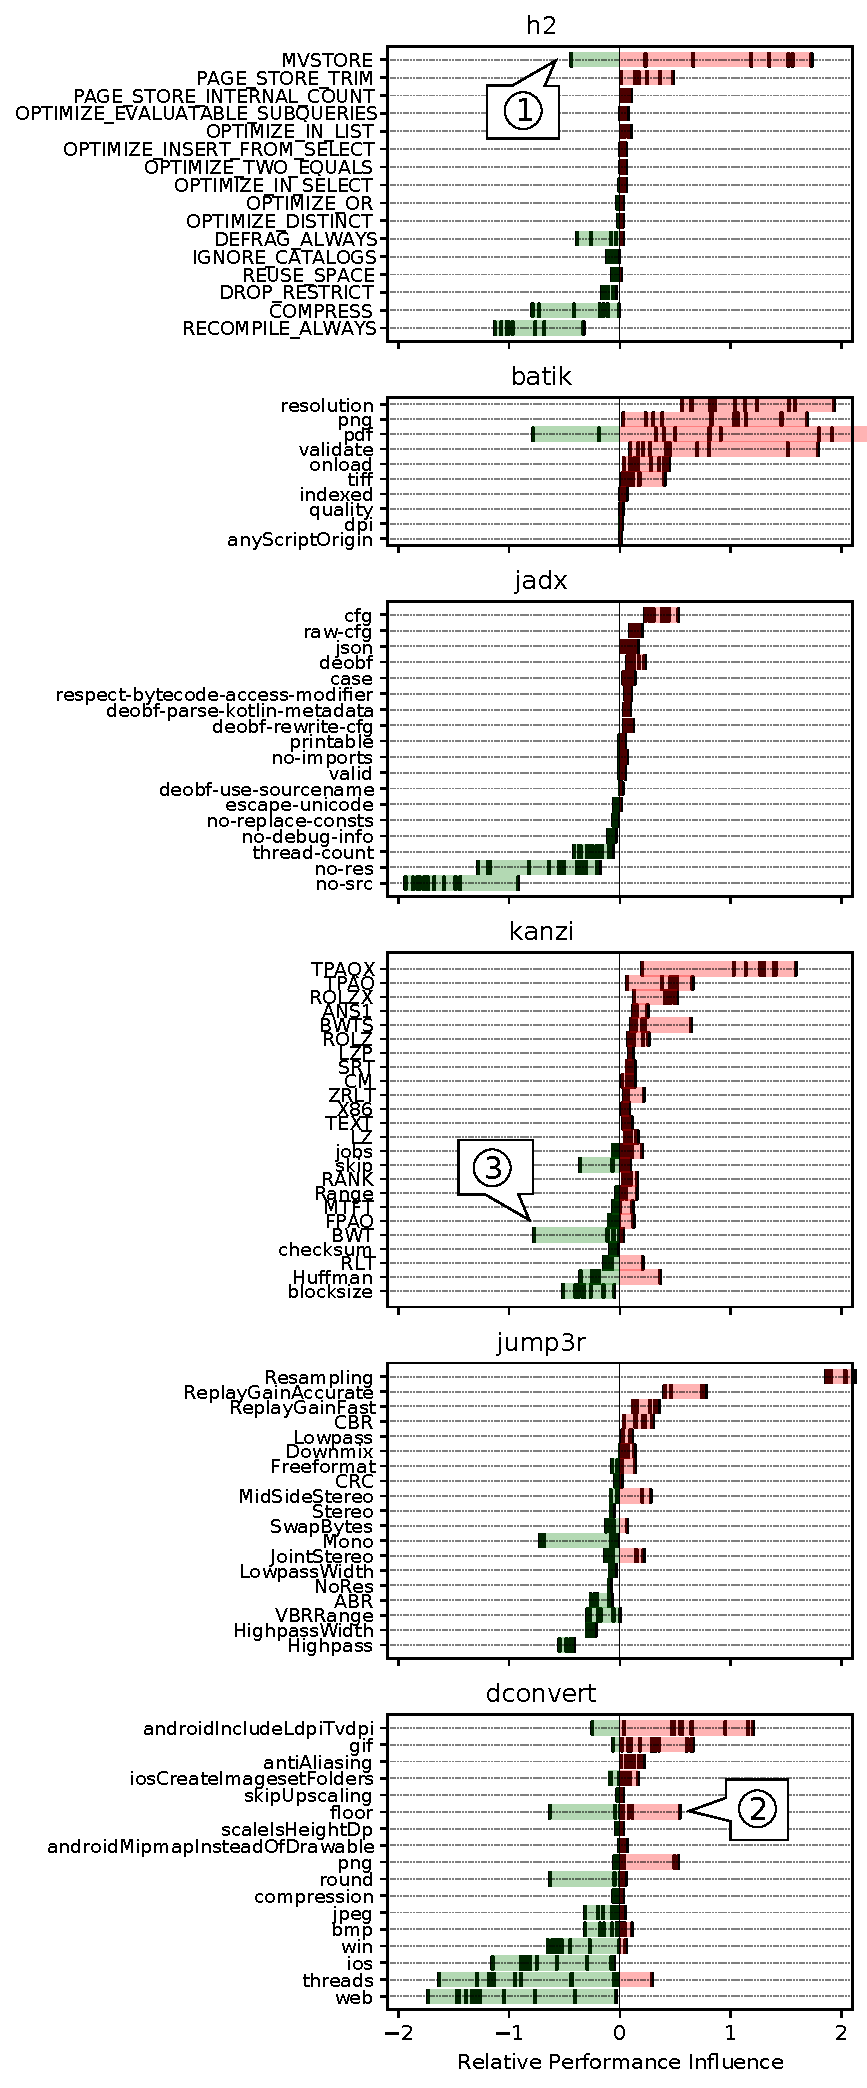
\includegraphics[width=0.97\linewidth]{images/out_annotated2.pdf}
	\caption{Relative performance influences (\textit{standardized regression coefficients}) for all configuration options across all workloads. Each black bar denotes a workload-specific performance influence. For each configuration option, we highlight the range of observed influences. }
	\label{fig:results_influence}
\end{figure}

We have identified three characteristic (but non-exclusive) traits, by which we can describe the distributions of regression coefficients: 
\begin{compactitem}	
\item[\circled{1}] \emph{Spread} of performance influences: Some distributions scatter over a wide range, while others are concentrated around a single value. Consider \htwo, for which we observe a relative performance difference of 200\,\% for option \textsf{MVSTORE}, meaning that the performance influence of turning on this option can be twice as high depending on the workload. 

\item[\circled{2}] \emph{Opposing influences}: Some distributions exhibit both positive and negative coefficients, while others remain consistent, either positive or negative. For \dconvert, we observe both positive and negative influences for option \textsf{floor} for two workloads, while for the remaining workloads, the option has neglible influence.

\item[\circled{3}] \emph{Conditional influences}: For some models, the majority of coefficients is negligible, but for few workloads we observe options having an influence. For example, for \kanzi, we observe for option \textsf{BWT} a negative influence only for a specific workload, whereas for all others the option has no influence.
\end{compactitem}
	
These criteria, the spread (\circled{1}) or concentration, opposing influences (\circled{2}), and options becoming influential only on occasions (\circled{3}), allow us to group each configuration option into a specific category, as presented in Table~\ref{tab:option_classification}. We omitted all configuration options with low spread and a neglible performance influence since these are not interacting with the workload either. 


\begin{table}[ht!]
	\centering
	\footnotesize
	\caption{Classification of relative performance influence distributions with respect to \textit{spread}, \textit{opposing influence}, and \textit{conditional influence.}}
	\begin{tabular}{p{1.2cm}p{0.7cm}rp{4.9cm}} % h2 batik jadx
		\toprule
		\textbf{Category} & \textbf{System} & \textbf{\#} & \textbf{Options} \\
		\midrule
		
		\multirow{5}{*}{\parbox{1.3cm}{ \centering \circled{1}\\\vspace{1mm} High Spread}} & \kanzi & 1 & \textsf{TPAQX}\\
		\cmidrule{2-4}
		& \dconvert & 6 & \textsf{androidIncludeLdpiTvdpi, gif, win, ios, threads, web} \\
		\cmidrule{2-4}
		& \htwo & 3 & \textsf{\mbox{RECOMPILE\_ALWAYS, MVSTORE}, \mbox{COMPRESS}} \\
		\cmidrule{2-4}
		& \batik & 4 & \textsf{resolution, png, pdf, validate}\\
		\cmidrule{2-4}
		& \jadx & 2 & \textsf{no-res, no-src}\\
		\midrule
		
		\multirow{5}{*}{\parbox{1.3cm}{\centering \circled{2}\\\vspace{1mm} Opposing Influences}} & \kanzi & 2 & \textsf{Huffman, RLT} \\
		\cmidrule{2-4}
		& \dconvert & 3 & \textsf{threads, androidIncludeLdpiTvdpi, floor} \\
		\cmidrule{2-4}
		& \htwo & 1 & \textsf{MVSTORE}\\
		\cmidrule{2-4}
		& \batik & 1 & \textsf{pdf}\\
		\midrule
		
		\multirow{5}{*}{\parbox{1.3cm}{\centering \circled{3}\\\vspace{1mm}Conditional Influences}} & \jumper & 3 & \textsf{Mono, MidSideStereo, JointStereo}\\
		\cmidrule{2-4}
		 & \kanzi & 4 & \textsf{BWT, skip, TPAQ, TPAQX} \\
		 \cmidrule{2-4}
		 & \dconvert & 7 & \textsf{floor, png, round, threads, web, ios, win} \\
		 \cmidrule{2-4}
		 & \htwo & 2 & \textsf{DEFRAG\_ALWAYS, COMPRESS} \\
		 \cmidrule{2-4}
		 & \batik & 3 & \textsf{onload, tiff, png}\\
		 
		\bottomrule
	\end{tabular}	
\label{tab:option_classification}
\end{table}

With two exceptions, we see that all software systems have configuration options, for which, at least, one of the three characteristic traits apply. For \jumper, we found only conditional influences for three options, whereas for \jadx, we observed only three options with high spread of relative performance influences. As these differences arise from varying the workload, we conclude that input sensitivity of a configuration option can manifest in different ways, as shown by the three characteristics.
\vspace{1mm}
\greybox{\color{red}\textbf{Summary} (\RQref{2}): Configuration options are profoundly input sensitive: We observe high performance variations, non-mo\-no\-to\-nic behavior, conditional influence, and even diametrically opposed influences for a single option.}
}

\end{comment}
\subsection{Code Coverage and Performance ($RQ_3$)}\label{sec:rq3}\label{sec:categories}
\subsubsection{Operationalization} From the findings of \RQref{2}, we have learned that input sensitivity of configuration options is specific to certain configuration options and can be diverse along multiple dimensions. With regard to the characteristic traits from~\RQref{2}, we conjecture that workload-specific sign flipping or conditional influences are driving factors for non-monotonicity across entire performance distributions (cf.~\RQref{1}). From these findings, the question arises: What causes these different aspects of input sensitivity? For a practical setting, one might, in addition, ask whether it is possible to identify input-sensitive configuration options without the effort of measuring substantial portions of the configuration space under varying worklods.
To shed light on possible explanations for input sensitivity, in general, and, possibly, different shades (cf.~\RQref{2}), we switch to the code level and analyze the relation of performance influences inferred for each configuration option to code coverage information. 

We augment our performance observations with code coverage information to assess differences in the execution under different workloads. Specifically, we are interested in code sections that implement option-specific functionality (i.e., functionality that is used only if the configuration option is selected). From comparing the coverage information of option-specific code, we can formulate different hypothetical scenarios explaining input sensitivity. 

First, if we observe that the  coverage of option-specific code is conditioned by the presence of some workload characteristic, we expect that such an option is only influential under respective workloads. This scenario enables us (to some extent) to use code coverage as a cheap-to-compute proxy for estimating the representativeness of a workload and, by extension, resulting performance models: For options that are known to condition code sections, we can maximize option-code coverage to elicit all option-specific behavior and, thus, performance influence. For instance, a database system could cache a specific view only if a minimum number of queries are executed. Here, the effect of any caching feature would be conditioned by the number of transactions resulting from the workload.

Second, if we observe performance variation across workloads in spite of similar or identical option-specific code coverage, we draw a different picture. Here, we cannot attribute performance variation to code coverage, yet have to consider differences in the workloads’ characteristics as potential cause: The presence of a workload characteristic may influence not  \emph{what} code sections are executed, but \emph{how} code sections are executed. For instance, in a simple case, a software system’s performance may scale linearly with the input size. In a more complex case, the presence of a characteristic may determine how frequently an operation is repeated, as is the case for a database merge. Here, we would not elicit the worst-case performance if a previous transaction has sorted the data (e.g., by building an index).

\subsubsection{Locating Configuration-Dependent Code}
To reason about option-specific code, we require a mapping of configuration options to code. 
The problem of determining which code section implements which functionality in a software system is known as \emph{feature location}~\cite{rubin_feature_2013}. 
While there are a number of approaches based on static~\cite{velez_2020_configcrusher_jase,lillack_2018_lotrack_tse,luo_2019_cova} and dynamic taint analysis~\cite{bell_phosphor_2014,velez_comprex_2021,splat_kim_2013}, we employ a more light-weight,  but also less precise approach that uses code coverage information, such as execution traces.
The rationale is that, by exercising feature code, for instance via enabling configuration options or running corresponding tests, its location can be inferred from differences in code coverage. 
Applications of such an approach have been studied not only for feature location~\cite{wong_integrated_2005,sulir_annotation_2015,michelon_spectrum_2021,perez_framing_2016}, but root work on in program comprehension~\cite{wilde_early_1996,wilde_reconnaissance_1995,sherwood_reducing_nodate,perez_diagnosis_2014,castro_pangolin_2019} and fault localization~\cite{agrawal_fault_1995,wong_faultloc_2016}. 
}
Specifically, we follow  a strategy akin to  \textit{spectrum-based feature location}~\cite{michelon_spectrum_2021}:
First, we obtain a baseline of \textit{all} option code in the scope of the entire workload selection. For each workload $w \in W$, we compute the set of code lines that depend on any option $o \in O$. 
Let $C_{o}$ be the set of configurations with option $o$ selected, and $C_{\neg o}$ with option $o$ deselected. To obtain the code sections specific to option $o$ under workload $w$, $S_{w, o}$, we subtract the set of the code lines covered under $C_{\neg o}$ from those of $C_{o}$:
\begin{equation}%\todo{example from Figure~\ref{fig:intro}}
	S_{w, o} = \bigcup_{p \in C_{o}} S_{w}(p) ~ \setminus ~ \bigcup_{q \in C_{\neg o}} S_{w}(q)
\end{equation}
While $S_{w, o}$ yields an approximation of option-dependent code for a single workload, we aggregate the approximations for each workload $w\in W$ to obtain the set of lines that depend on a configuration option $o$ and are executed in, at least, one workload,~$S_{o}$: 
\begin{equation}
	S_{o} = \bigcup_{w \in W} S_{w, o}
\end{equation}
While this aggregated set is not a ground truth per se, it enables us to reason about differences in option-dependent code in the scope of our selected workloads. That is, the expressiveness of this baseline depends on the diversity of the workloads in question. From the ratio of option-specific code per workload to option-specific code across workloads, $\mid S_{w_1, o}\mid/~{\mid S_{w_2, o}\mid}$, we can estimate the coverage of option-dependent code. 

\subsubsection{Comparing Execution Footprints}
From (a) the information about which code sections are specific to a configuration option and (b) how much of these sections is actually covered under different workloads, we can compare the workload-specific execution footprint for each option. By comparing the sets $S_{w_1, o}$ and $S_{w_2, o}$ for any two workloads $w_1$ and $w_2$, we can estimate similarity between the option-code coverage via the Jaccard set similarity index. A Jaccard similariy of zero implies that there is no overlap in the lines covered under each workload, whereas a Jaccard similarity of 1 implies that the exact same code was covered. Based on this pairwise similarity metric $sim_o(w_1, w_2)$, we can compute a distance $d_o(w_1, w_2) = 1 - sim(w_1, w_2)$ and cluster all workload-specific execution profiles. 

We use agglomerative hierarchical clustering with full linkage to construct dendrograms, as shown in Figure~\ref{fig:results_rq3}. In this bottom-up approach, we iteratively add execution footprints to clusters and merge sub clusters into larger ones depending on their Jaccard similarity  to each other. The vertical bars with respect to the x-axis denote the Jaccard distance between merged clusters or, for initial clusters, constituent execution footprints. Finally, we compare (a) the clustering of workload-specific execution profiles for each option with (b) the distribution of relative performance influences for the respective option. As a recap, the distribution of performance influences refers to individual rows in Figure~\ref{fig:results_influence}. In essence, we ask whether variation in the observed distribution of relative performance influences correspond to similarities or differences in what, or what portions of, option-specific code is executed. Of special interest are the patterns identified in Section~\ref{sec:results2} and the involved configuration options from Table~\ref{tab:option_classification}.

\subsubsection{Results}
\begin{comment}
We inspected manually the relation of the coverage similarity across workloads per option and the observed workload-specific performance influences.  For the majority of cases, the results suggest that the workload determines how the code is executed since we did not observe a strong relationship between performance variation and differences in code coverage. However, we have identified seven configuration options across three software systems (\jumper, \kanzi, and \dconvert) for which code coverage is likely the driving factor for performance variation. We present illustrative examples for both scenarios in Figure~\ref{fig:results_rq3}.
\begin{figure}
	
	\centering
	\begin{subfigure}{0.99\linewidth}
		\begin{minipage}{0.5\linewidth}
			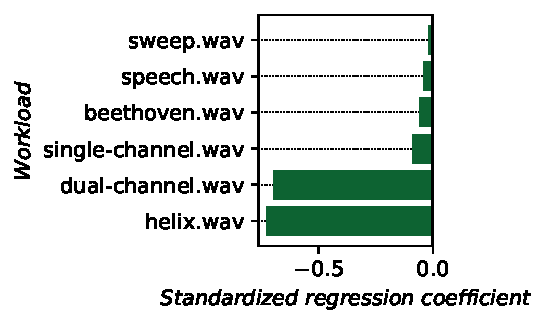
\includegraphics[width=\linewidth]{images/plots/jump3r_Mono_influences.pdf}
		\end{minipage}
		\begin{minipage}{0.5\linewidth}
			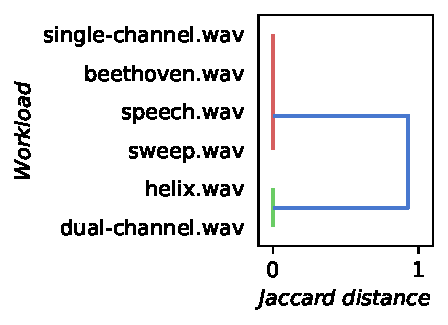
\includegraphics[width=0.9\linewidth]{images/plots/jump3r_Mono_workloads.pdf}
		\end{minipage}
		\caption{Configuration option \guillemotleft\textsf{Mono}\guillemotright~of \jumper}
		\label{fig:results_rq3_jump3r}
	\end{subfigure}
	
	\begin{subfigure}{0.99\linewidth}
		\begin{minipage}{0.5\linewidth}
			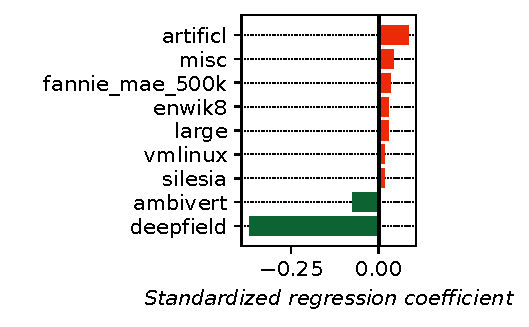
\includegraphics[width=\linewidth]{images/plots/kanzi_skip_influences.pdf}
		\end{minipage}
		\begin{minipage}{0.5\linewidth}
			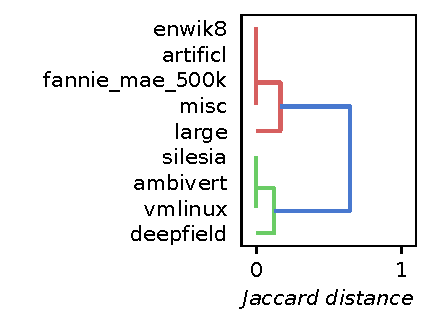
\includegraphics[width=0.9\linewidth]{images/plots/kanzi_skip_workloads.pdf}
		\end{minipage}
		\caption{Configuration option \guillemotleft\textsf{skip}\guillemotright~ of \kanzi}
		\label{fig:results_rq3_kanzi}
	\end{subfigure}

	\begin{subfigure}{0.99\linewidth}
		\begin{minipage}{0.5\linewidth}
			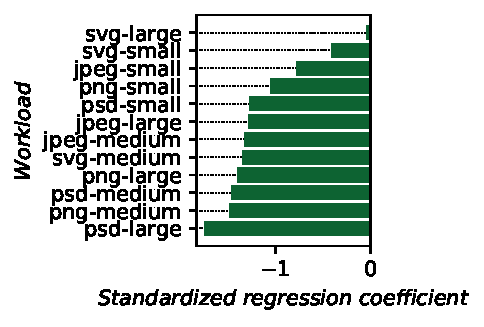
\includegraphics[width=\linewidth]{images/plots/dconvert_web_influences.pdf}
		\end{minipage}
		\begin{minipage}{0.5\linewidth}
			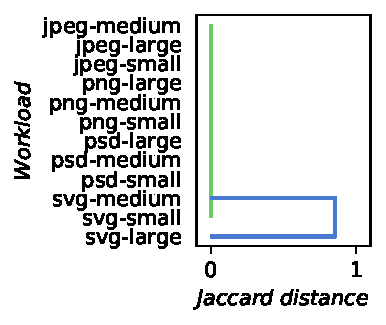
\includegraphics[width=0.9\linewidth]{images/plots/dconvert_web_workloads.pdf}
		\end{minipage}
		\caption{Configuration option \guillemotleft\textsf{web}\guillemotright~ of \dconvert}
		\label{fig:results_rq3_dconvert}
	\end{subfigure}
	
	\begin{subfigure}{0.99\linewidth}
		\begin{minipage}{0.5\linewidth}
			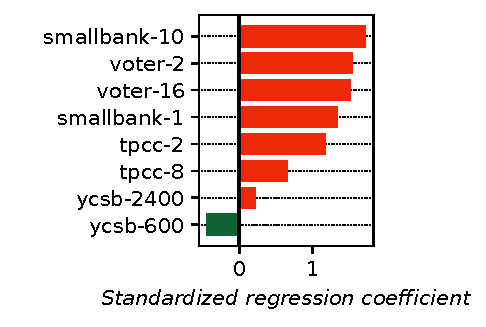
\includegraphics[width=\linewidth]{images/plots/h2_MVSTORE_influences.pdf}
		\end{minipage}
		\begin{minipage}{0.5\linewidth}
			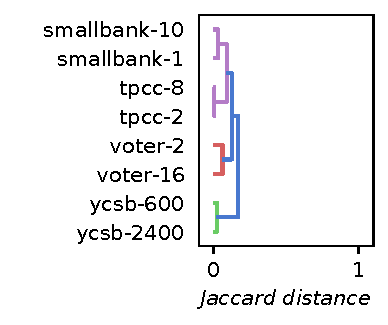
\includegraphics[width=0.9\linewidth]{images/plots/h2_MVSTORE_workloads.pdf}
		\end{minipage}
		\caption{Configuration option \guillemotleft\textsf{COMPRESS}\guillemotright~ of \htwo}
		\label{fig:results_rq3_h2}
	\end{subfigure}
	\caption{\color{red}Distribution of relative performance influences across workloads (left) and cluster dendrogram of workload-specific option-code executions (right).}
	\label{fig:results_rq3}
\end{figure}

For the scenario of a workload conditioning code coverage, \jumper is a good illustrative example in Figure~\ref{fig:results_rq3_jump3r}: We have identified two workloads that exhibit multiple audio channels (\textsf{helix.wav} and \textsf{dual-channel.wav}) under which configuration options (\textsf{Mono, MidSideStereo and JointStereo}) become influential. This is supported by the coverage information we collected, where we see that both workloads result in similar code sections covered, whereas such code sections are not covered under other workloads. We observe similar effects for \kanzi and \dconvert. For \kanzi, we find two distinct clusters of code coverage whose workloads show opposing influences for option \textsf{skip} (cf. Figure~\ref{fig:results_rq3_kanzi}). For \dconvert, under workload \textsf{svg-large} no option-specific code is executed, resulting in little influence for options \textsf{web, ios, and gif} (cf. Figure~\ref{fig:results_rq3_dconvert}). These three examples suggest that a workload can indeed determine whether a configuration option's code section is executed and thus determine whether this option is influential and whether its performance influence is positive or negative. 

By contrast, the majority of cases we inspected did not show such a relationship. We illustrate one example that highlights that non-linear shifts in performance influence can arise even from little differences in the workload. For \htwo, we pursued a rather controlled experiment. Here, we vary the scale factor for four different standard benchmarks. Thus, we can expect some inherent similarity across these pairs. In Figure~\ref{fig:results_rq3_h2}, we show the comparison of performance influences and the corresponding dendrogram for the configuration option \textsf{COMPRESS}. While we see that the execution footprints for the pairs of benchmarks form clusters and are quite similar (i.e., the distance is below 0.3 among all workloads), we still observe considerable performance variation, most notably, in the case of workload \textsf{ycsb-600}. So, contrary to our expectation, varying only one characteristic (here, the scale factor) can introduce further variation that cannot be plausibly explained by workload-specific code coverage. 

For the other subject systems and remaining configuration options, we could not find any relation between workload-dependent performance variations and code coverage. We found both cases, differences in code coverage do not correspond to variation in the relative performance influences and vice versa. That is, for the majority of configuration options, input sensitivity cannot be explained by a varying option-specific code coverage. Instead, workload characteristics most likely account for variation in how covered option specific-code is executed, including the loop passes and method calls as well as variation arising from method arguments.
\vspace{1mm}
\greybox{\textbf{Summary} (\RQref{3}): Varying the workload can condition the execution of option-specific code  (\textit{code coverage}) and cause performance differences. However, there is no single driving factor: \textit{Code utilization} depending on workload characteristics is a likely factor accounting for the majority of performance influence variation.  
}
\end{comment}
\todo{Here results from RQ3}
%\clearpage
\section{Discussion}

\subsection{Option-level Input Sensitivity}

The observed input sensitivity for configuration options exhibits a wide range of characteristics. While a large portion of options scales proportionally with workload complexity or remains unaffected by workload variation, the performance influences of several configuration options appear sensitive to the workload.  So far, the existing body of work on modeling and optimizing configuration-specific performance largely neglects the impact of workload variation at the cost of generalizability. Option-specific input sensitivity is a strong motivation for assessing influential factors beyond configuration options more thoroughly and rigorously. Performance variation that is unaccounted for poses the risk of distorting performance estimations and, thus, rendering performance models useless in practice. Although transfer learning is used in literature to reuse existing performance models across different workloads, our findings let us raise concerns about its effectiveness and generalizability. 

In their exploratory analysis, Jamshidi et al. reuse existing performance models by learning a linear transfer function across workloads~\cite{jamishidi_transfer_2017}. Our results from \RQref{1} have shown non-monotonous performance relationships across workloads, which, in practice, can be challenging to capture with such transfer functions. The presence of \textit{non-monotonous interactions} between workloads and configuration options provides a strong argument for employing more apt machine learning techniques. Ensemble-based approaches, such as gradient boosting regression trees have shown promising results for transfer across versions and are an avenue for future work~\cite{martin_transfer_2021}.

\greybox{\textbf{Summary:} Option-level input sensitivity can challenge robust and practical configuration-specific performance models, yet is neglected in state-of-the-art approaches.
}

\subsection{Driving Factors for Input Sensitivity}
Extending on the findings from RQ2 and RQ3, to treat option-specific input sensitivity, a key challenge is to infer which options are susceptible to workload variation. Despite the limitations faced with the coverage-based approach from RQ3 (missing baseline), we have correlated missed option code with variation in the observed performance. Our findings point to more detailed code analysis, such as line hit counts or execution logs, and more profound domain knowledge as key ingredients for mastering the input sensitivity assessment. In literature, the heuristic to consider only influential configuration options for transfer learning has shown effective results~\cite{jamshidi_learning_2018}. However, we question whether this approach would generalize in practice in the light of the conditional performance influences observed in Setions~\ref{sec:rq2} and \ref{sec:rq3}. Clearly, more research is needed to provide an empirical base and framework for sensitivity assessment.

\greybox{\textbf{Summary:} Understanding the driving factors for input sensitivity is necessary for providing representative workloads and identifying sensitive configuration options. 
}

\section{Threats to Validity}\label{sec:threats}

Threats to \textit{internal validity} include measurement noise which may distort our classification into categories (Section~\ref{sec:rq1}) and model construction (Section~\ref{sec:rq2}). We mitigate these threats by repeating each experiment five times  (except for \htwo; cf. Section~\ref{sec:measurement_setup}) and reporting the median as a robust measure in a controlled environment. Moreover, the coverage analysis (cf. Section~\ref{sec:profiling}) entails a noticeable instrumentation overhead, which may distort performance observations. We mitigate this threat by separating the experiment runs for coverage assessment and performance measurement. In the case of \htwo, the load generator of the \textsc{OLTPBench} framework~\cite{difallah_oltp_2013} ran on the same machine as the database since we were testing an embedded scenario with only negligible overhead. 	
	
Threats to\textit{ external validity} include the selection of subject systems and workloads. To ensure generalizability, we select software systems from various various application domains as well as two different programming language ecosystems (cf.~Table~\ref{tab:subject_systems}). In lieu of domain knowledge, we cannot select workloads systematically with respect to workload characteristics due to workloads inherent opacity. We address this issue by varying likely relevant characteristics and, where possible, reusing workloads across subject systems of the same domain. Achieving true representativeness is desirable, yet intractable. 
The goal of this selection is to study the \emph{presence} and quality of workload-option interactions, but not their \emph{prevalence}. Hence, we are confident that this selection does not invalidate our findings.

{\color{magenta}Threats to \textit{construct validity} include our choice of correlation metrics in Section~\ref{sec:rq1}, regression technique in Section~\ref{sec:rq2}, and similarity metric in Section~\ref{sec:rq3}. The correlation metrics are widely used to describe statistical relationships and the overall picture remains consistent with slightly different thresholds. Multiple linear regression as well 
}
\color{black}
\section{Conclusion}\label{sec:conclusion}
Most modern software systems exhibit configuration options to customize behaviors and meet user demands. Configuration choices, however, can also affect the performance of a software system.
State-of-the-art approaches model configuration-dependent software performance, yet overlook variation due to the workload. Until now, there exists no \textit{systematic} assessment of what is driving the effect that input sensitivity of individual configuration options’ influence on performance. We have conducted an empirical study of {\color{red}35\,659 configurations and 103 workloads across ten} configurable software systems to characterize the effects that varying the workload can have on configuration-specific performance. We compare performance measurements with code coverage data to identify possible factors that drive input sensitivity. We found that the interactions between options and workloads are driven by workload characteristics conditioning the execution of option-specific code sections as well as determining how option-specific code sections are executed. Our findings highlight the necessity to consider input sensitivity when modeling configuration-dependent performance as varying the workload resulted in a substantial number of non-monotonous relationships, which limits a performance model's representativeness. Code analysis can provide an effective strategy to differentiate between sources of input sensitivity to obtain more representative performance models.

